\documentclass[12pt]{article}
\usepackage[utf8]{inputenc}
\usepackage[a4paper, margin=2cm]{geometry}
\usepackage{amsthm}
\usepackage{amsmath, amssymb}
\usepackage{circuitikz}
\usepackage{graphicx}
\usepackage{karnaugh-map}
\usepackage{newtxtext, newtxmath}
\usepackage{tcolorbox}
\usepackage{tikz}
\usepackage{titlesec}
\usepackage{xcolor}
\usepackage{xeCJK}
\usepackage{listings}
\definecolor{lightblue}{RGB}{135, 206, 250}
\tcbuselibrary{skins,theorems}

\titleformat{\section}[block]{\Large\bfseries\centering}{}{0pt}{}
\titleformat{\subsection}[block]{\bfseries}{\thesubsection}{2pt}{}

\newtcbtheorem[no counter]{proposition}{\large\hspace{-8pt}Proposition}{
  enhanced,
  colback=white,
  colframe=lightblue,
  left=12pt,
  right=12pt,
  top=24pt,
  bottom=24pt,
  fonttitle=\bfseries
}{prop}
\newtcbtheorem[]{question}{\large\hspace{-8pt}Question :}{
  enhanced,
  colback=white,
  colframe=black,
  left=12pt,
  right=12pt,
  top=24pt,
  bottom=24pt,
  fonttitle=\bfseries
}{qst}
\newenvironment{Answer}{
  \vspace{12pt}
  {\large\textbf{\textit{\hspace{-12pt}Answer:}}}\par
  \vspace{8pt}
} {\vspace{24pt}}
\newenvironment{Proof}{
  \vspace{12pt}
  {\large\textbf{\textit{\hspace{-12pt}Proof:}}}\par
  \vspace{8pt}
} {\vspace{24pt}}

\lstset{
    language=Python,
    basicstyle=\ttfamily\footnotesize,
    keywordstyle=\color{blue}\bfseries,
    commentstyle=\color{gray},
    stringstyle=\color{red},
    showstringspaces=false,
    numberstyle=\tiny\color{gray},
    stepnumber=1,
    numbersep=10pt,
    frame=single,
    breaklines=true,
    captionpos=b
}

\title{\textbf{Introduction to IoT Homework 1}}
\date{September 10, 2024}

\begin{document}
\maketitle

\begin{question}{}{}
1、列出、介绍手机使用到的传感器。
\end{question}
\begin{Answer}

\subsection*{引言}\noindent

在当今的智能手机中，
传感器技术发挥了至关重要的作用，
使得设备能够感知、交互和适应周围环境。
传感器的应用不仅提升了用户体验，
还为各种新型功能提供了技术支持。
从检测设备的运动状态，到精确的生物识别，
手机传感器极大丰富了移动设备的功能性，
令智能手机从一个简单的通信工具，
发展为一款集多种智能功能于一体的设备。

智能手机中集成的传感器种类繁多，
包括运动传感器、环境传感器、生物识别传感器、成像与视觉传感器、接近和触控传感器以及声音与振动传感器。
这些传感器通过实时监测环境信息并将其转化为可处理的数据，
帮助手机执行各种复杂的任务。
例如，陀螺仪和加速度计共同工作，
能够感知设备的移动和方向变化；
而指纹传感器和面部识别传感器则极大提高了设备的安全性。

\begin{figure}[htbp]
    \centering
    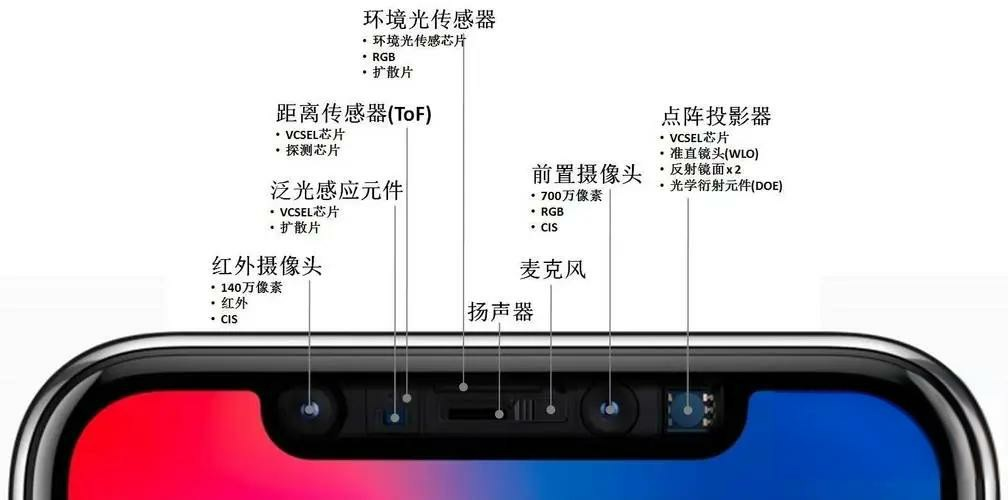
\includegraphics[width=0.8\textwidth]{image/1_1.jpg}
    \caption{手机各种传感器展示}
\end{figure}

随着科技的进步，
手机传感器的性能不断提升，
未来的传感器将会更加微型化、集成化，
并应用于更多元的场景中，
例如物联网设备和健康监测领域。
本文将详细介绍手机中使用到的各类传感器，
分析它们的工作原理及实际应用场景，
帮助我们更好地理解这些传感器的作用及其发展趋势。

\subsection*{运动传感器}\noindent

智能手机中的运动传感器用于检测设备的移动、方向和加速度，
帮助设备感知其在空间中的位置和运动状态。
主要的运动传感器包括加速度计、陀螺仪和磁力计。
这些传感器通常协同工作，
为各种功能提供数据支持，
如自动屏幕旋转、步数计数、导航和增强现实（AR）应用等。

\begin{figure}[htbp]
    \centering
    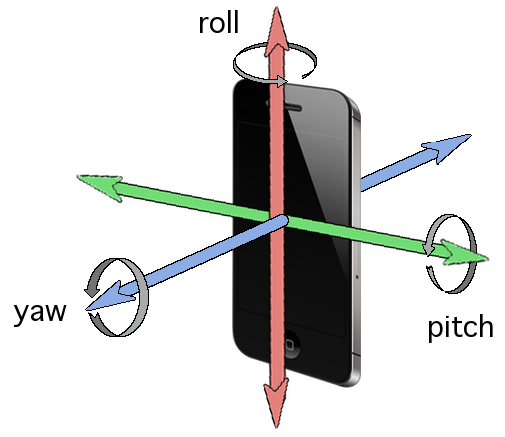
\includegraphics[width=0.8\textwidth]{image/1_2.png}
    \caption{手机运动传感器原理}
\end{figure}

\noindent\textbf{1. 加速度计}\noindent

加速度计（Accelerometer）是智能手机中最常用的运动传感器之一，
能够测量设备在三维空间中的线性加速度。
通过检测施加在手机上的重力方向和大小，
加速度计可以确定手机的方位和移动速度。
常见的应用包括自动屏幕旋转、步数记录、震动检测以及用户运动追踪等。

\textbf{应用场景}：
\begin{itemize}
    \item \textit{自动屏幕旋转}：加速度计通过感知设备的方向变化，自动调整屏幕显示的方向。
    \item \textit{健康与运动追踪}：结合软件算法，加速度计可用于记录步数、运动距离和卡路里消耗。
    \item \textit{游戏控制}：在一些运动感应游戏中，加速度计可以检测用户的手机移动，提供游戏控制输入。
\end{itemize}

\noindent\textbf{2. 陀螺仪}\noindent

陀螺仪（Gyroscope）是另一种常见的运动传感器
它可以测量设备的角速度和旋转方向。与加速度计不同，
陀螺仪主要检测设备的旋转运动，
尤其是旋转速度和角度的变化。
加速度计与陀螺仪通常结合使用，
提供更精确的设备方向和运动数据，
特别是在需要精确控制的应用中，
如增强现实（AR）和虚拟现实（VR）应用。

\textbf{应用场景}：
\begin{itemize}
    \item \textit{增强现实（AR）和虚拟现实（VR）应用}：陀螺仪帮助设备精确感知用户的头部和身体旋转，增强了AR和VR体验的沉浸感。
    \item \textit{游戏中的精确控制}：在许多赛车和动作游戏中，陀螺仪为手机提供了精准的方向和角速度检测，使游戏控制更加灵活。
    \item \textit{视频防抖}：在摄像应用中，陀螺仪通过检测设备的抖动和旋转，帮助减轻视频录制过程中的抖动，提升视频质量。
\end{itemize}

\noindent\textbf{3. 磁力计（电子罗盘）}\noindent
磁力计（Magnetometer），也称为电子罗盘，
是手机中用来探测地球磁场方向的传感器。
它能够识别设备相对于地球磁场的方位，
因此在导航应用中起到了关键作用。
与加速度计和陀螺仪配合使用，
磁力计能够帮助手机在三维空间中定位自身方向，
使得地图应用中的指南针功能得以实现。

\textbf{应用场景}：
\begin{itemize}
    \item \textit{导航和定位}：磁力计为地图和导航应用提供准确的方向指引，帮助用户在开车或步行时保持正确的行进方向。
    \item \textit{增强现实（AR）}：在AR应用中，磁力计与其他传感器协同工作，提供精确的方向感知，增强虚拟与现实的互动体验。
\end{itemize}

\noindent\textbf{4. 运动传感器的协同工作}\noindent

加速度计、陀螺仪和磁力计通常协同工作，
以提供更加准确和全面的运动数据。
它们共同构成了惯性测量单元（IMU），
广泛应用于手机的导航、运动追踪、游戏和增强现实等功能。
这些传感器结合起来，
为手机提供了丰富的运动感知能力，
从而为用户带来了更高精度的定位和交互体验。

\subsection*{环境传感器}\noindent

环境传感器在智能手机中用于检测和监控周围环境的物理条件。
它们能够提供关于光线、气压、温度、湿度等信息，
帮助设备根据环境变化调整自身设置，
从而提升用户体验和设备性能。
常见的环境传感器包括环境光传感器、气压计、温度传感器和湿度传感器。

\noindent\textbf{1. 环境光传感器}\noindent

环境光传感器（Ambient Light Sensor）用于检测周围环境中的光线强度。
根据测得的光照数据，
智能手机可以自动调整屏幕的亮度，
以适应不同的光照条件，从而提供更好的显示效果，
并在强光下提高可读性，
或在暗光下减低亮度以节省电能。

\textbf{应用场景}：
\begin{itemize}
    \item \textit{自动亮度调节}：根据环境光的变化，自动调整手机屏幕的亮度，既节省电池，又保证用户视觉舒适度。
    \item \textit{省电模式}：在低光条件下自动降低屏幕亮度，延长电池寿命。
\end{itemize}

\noindent\textbf{2. 气压计}\noindent

气压计（Barometer）是一种用于测量大气压力的传感器。
在手机中，气压计主要用于提高GPS系统的高度测量精度。
通过检测大气压力的变化，设备可以更准确地估算当前的海拔高度，
这在户外活动中尤为重要，
例如登山或飞行模式下的高度追踪。
此外，气压计还可以为天气预报应用提供本地大气压力数据，
帮助预测短期天气变化。

\textbf{应用场景}：
\begin{itemize}
    \item \textit{提高GPS定位精度}：通过气压计提供的高度数据，结合GPS信息，手机可以更精确地定位使用者的垂直位置。
    \item \textit{户外运动跟踪}：对于登山和户外运动爱好者，气压计可以提供海拔变化的实时数据。
    \item \textit{天气预报}：气压计为天气应用提供本地的气压变化信息，帮助更准确地预测短期天气变化。
\end{itemize}

\noindent\textbf{3. 温度传感器}\noindent

温度传感器（Temperature Sensor）用于检测手机内部或周围环境的温度。
虽然大多数智能手机不直接对用户公开温度数据，
但该传感器在设备内部用于监控手机的运行温度，
防止过热对设备造成损害。
当设备温度超过一定阈值时，
系统会自动调整处理器性能或提示用户关闭一些高耗能的应用，
以避免设备损坏。

\textbf{应用场景}：
\begin{itemize}
    \item \textit{设备过热保护}：监控手机的温度，在设备温度过高时自动降低处理器频率，避免硬件损坏。
    \item \textit{环境监测}：一些设备和应用使用温度传感器来检测周围的环境温度，为用户提供天气或健康相关的数据。
\end{itemize}

\noindent\textbf{4. 湿度传感器}\noindent

湿度传感器（Humidity Sensor）用于测量环境中的湿度。
虽然不常见于大多数智能手机中，
但一些专用设备或高端手机可能配备湿度传感器，
用于环境监测或健康追踪应用。
该传感器可帮助用户了解当前环境的湿度水平，
对于需要保持特定湿度的场景（如实验室或温室）尤为重要。

\textbf{应用场景}：
\begin{itemize}
    \item \textit{环境监控}：用于检测房间或周围环境的湿度水平，帮助用户在不适的湿度条件下调整环境。
    \item \textit{健康应用}：结合温度和湿度数据，某些健康应用可以提醒用户当前的环境是否适合户外活动或进行运动。
\end{itemize}

\noindent\textbf{5. 环境传感器的作用}\noindent

环境传感器为智能手机的环境感知能力提供了强有力的支持。
通过收集光线、气压、温度和湿度等数据，
这些传感器使设备能够动态适应不断变化的环境，优化用户体验。
无论是自动调整屏幕亮度，
还是提供更准确的GPS定位，
这些传感器的存在让手机更智能、更高效。

\subsection*{生物识别传感器}\noindent

生物识别传感器通过采集人体的独特生物特征（如指纹、面部、虹膜等）进行身份验证，
是现代智能手机安全领域的重要组成部分。
这类传感器的引入极大地提升了手机的安全性和便利性，
同时也推动了移动支付和个人隐私保护的发展。
常见的生物识别传感器包括指纹传感器、面部识别传感器和心率传感器。

\noindent\textbf{1. 指纹传感器}\noindent

指纹传感器（Fingerprint Sensor）是手机中最早普及的生物识别传感器之一。
它通过检测并分析用户指纹的细微特征来验证身份，
确保只有授权用户能够访问设备。
指纹传感器最早被集成在手机的物理按键中，
随着技术的发展，许多智能手机现在使用屏下指纹识别技术，
不仅提升了用户体验，还增加了手机的设计美感。

\textbf{应用场景}：
\begin{itemize}
    \item \textit{设备解锁}：用户可以通过轻触指纹传感器快速解锁设备，无需输入密码或图形。
    \item \textit{移动支付}：指纹传感器被广泛应用于移动支付，提供安全、高效的支付认证方式，减少了传统密码的繁琐。
    \item \textit{应用授权}：某些应用程序（如银行或加密软件）使用指纹传感器来验证用户身份，确保隐私数据的安全。
\end{itemize}

\noindent\textbf{2. 面部识别传感器}\noindent

面部识别传感器（Facial Recognition Sensor）是另一种常见的生物识别技术，
利用摄像头与3D结构光或红外线技术来捕捉和分析用户面部的特征。
这种传感器基于生物特征学，
通过匹配存储的面部数据来进行身份验证，
常用于设备解锁和安全支付。
与指纹传感器相比，面部识别技术通常更加直观和无接触式，
特别是在某些特定场景（如戴手套时）具有优势。

\textbf{应用场景}：
\begin{itemize}
    \item \textit{安全解锁}：面部识别技术通过扫描用户的面部特征，实现快速、无接触的设备解锁。
    \item \textit{支付验证}：类似于指纹传感器，面部识别也广泛用于支付场景中，提供安全可靠的支付认证方式。
    \item \textit{应用授权}：面部识别可以用于特定应用的访问控制，增强了应用的安全性。
\end{itemize}

\noindent\textbf{3. 心率传感器}\noindent

心率传感器（Heart Rate Sensor）通过光电容积描记法（PPG）测量用户的心率。
该传感器通常位于手机的背面或与智能手表等可穿戴设备集成，
通过检测血液流动的变化来计算心率。
尽管心率传感器在大多数情况下用于健康追踪，
但也可以作为辅助的生物识别工具，
结合其他生物特征验证用户身份。

\textbf{应用场景}：
\begin{itemize}
    \item \textit{健康监测}：心率传感器可以实时监控用户的心率，帮助用户跟踪健康状况，特别是在运动或高强度活动期间。
    \item \textit{压力管理}：一些应用结合心率数据来评估用户的压力水平，提供减压建议。
    \item \textit{身份验证}：心率传感器可以作为多重身份验证的一部分，增加设备或应用的安全性。
\end{itemize}

\noindent\textbf{4. 生物识别传感器的协同作用}\noindent

在现代智能手机中，指纹传感器、面部识别传感器和心率传感器等生物识别技术通常协同工作，
提供更高效、更安全的身份验证方式。
例如，一些设备支持同时使用指纹识别和面部识别来增强安全性，
而心率传感器则主要用于健康应用中的身份验证。
随着生物识别技术的不断进步，
未来将看到更多结合不同生物特征的复合身份验证方式，
为用户提供更安全、便捷的体验。

\subsection*{成像与视觉传感器}\noindent

成像与视觉传感器是现代智能手机中不可或缺的组成部分，
尤其随着移动摄影和视频记录需求的增长，
这类传感器变得越来越先进。
这些传感器不仅用于拍摄照片和视频，
还支持增强现实（AR）、虚拟现实（VR）等功能。
主要的成像与视觉传感器包括摄像头传感器、深度传感器和光谱传感器。

\noindent\textbf{1. 摄像头传感器}\noindent

摄像头传感器（Camera Sensor）是智能手机最重要的成像组件之一，
它通过将光线转换为电子信号来捕捉图像和视频。
现代智能手机通常配备多个摄像头传感器，
涵盖广角、超广角、长焦等不同焦段，以应对各种拍摄需求。
近年来，摄像头传感器的像素数、成像质量和动态范围得到了显著提升。

\textbf{应用场景}：
\begin{itemize}
    \item \textit{摄影与录像}：摄像头传感器用于拍摄高质量的照片和视频，尤其在夜景模式、人像模式和HDR摄影中发挥重要作用。
    \item \textit{增强现实（AR）应用}：通过摄像头传感器捕捉周围环境并将虚拟物体叠加在现实世界上，实现AR体验。
    \item \textit{二维码和条形码扫描}：摄像头传感器可以用于识别和解码二维码和条形码，在支付和产品信息获取方面广泛应用。
\end{itemize}

\noindent\textbf{2. 深度传感器}\noindent

深度传感器（Depth Sensor）通过检测物体与手机之间的距离来提供深度信息。
这类传感器通常采用飞行时间（ToF）技术、结构光技术或双摄像头的立体视觉来获取场景的深度数据。
深度传感器在拍摄时可以帮助分离背景和前景，
尤其在人像模式中，能够实现背景虚化效果，提供更专业的拍摄体验。

\textbf{应用场景}：
\begin{itemize}
    \item \textit{人像模式拍摄}：深度传感器用于拍摄时分离前景与背景，创造出类似单反相机的浅景深效果，实现背景虚化（“散景”）。
    \item \textit{增强现实（AR）应用}：在AR应用中，深度传感器帮助设备识别和感知真实世界的深度信息，提升虚拟物体与现实环境的互动效果。
    \item \textit{3D扫描}：深度传感器可以捕捉物体的三维形状，生成3D模型，用于虚拟现实、3D打印或其它需要精确测量的场景。
\end{itemize}

\noindent\textbf{3. 光谱传感器}\noindent

光谱传感器（Spectral Sensor）用于分析不同波长的光线，
这使得手机能够感知颜色的具体组成和光源的特性。
虽然光谱传感器目前在智能手机中的应用还不广泛，
但一些高端设备已经开始引入这一技术，
用于改善拍摄的色彩准确度，
甚至提供健康监测和环境检测功能。

\textbf{应用场景}：
\begin{itemize}
    \item \textit{色彩校准}：光谱传感器能够检测环境光的颜色偏差，帮助手机自动调整摄像头的白平衡和色彩呈现，提升照片和视频的色彩还原度。
    \item \textit{健康应用}：一些应用结合光谱传感器来分析皮肤状况或检测太阳光中紫外线的强度，帮助用户了解皮肤健康和防晒需求。
    \item \textit{环境监测}：光谱传感器能够检测环境光的成分，并为空气质量、污染或植物健康等应用提供支持。
\end{itemize}

\noindent\textbf{4. 成像与视觉传感器的协同作用}\noindent

现代智能手机通常结合使用摄像头传感器、深度传感器和光谱传感器，
以增强其成像和视觉处理能力。
例如，在拍摄模式中，摄像头传感器捕捉图像，
而深度传感器提供精确的景深信息，
实现专业级的虚化效果；
光谱传感器则能够调整色彩平衡，确保画面的真实还原。
这些传感器协同工作，
使智能手机成为功能强大的拍摄设备，
满足从日常摄影到复杂视觉处理的多种需求。

\subsection*{接近和触控传感器}\noindent

接近和触控传感器是智能手机中的重要组件，
用于增强用户与设备之间的交互体验。
接近传感器主要用于检测物体（如用户的手或面部）与设备的距离，
而触控传感器则检测用户在屏幕上的触摸动作。
这些传感器在日常使用中提供了诸多便捷功能，
如自动关闭屏幕、手势控制、多点触控等。

\noindent\textbf{1. 接近传感器}\noindent

接近传感器（Proximity Sensor）通常位于手机的前面板，
用于检测物体与设备之间的距离。
该传感器通过发射红外光线并检测其反射情况来判断物体的接近程度。
在日常使用中，接近传感器最常用于通话过程中，
检测用户的面部是否靠近屏幕，
从而自动关闭显示屏以避免误触并节省电能。

\textbf{应用场景}：
\begin{itemize}
    \item \textit{通话时自动关闭屏幕}：当用户将手机靠近耳朵时，接近传感器会关闭屏幕，防止误触，并节约电量。
    \item \textit{放入口袋时自动锁屏}：当手机放入口袋或包中时，接近传感器可以检测到遮挡，并自动关闭或锁定屏幕，防止误操作。
    \item \textit{手势操作}：部分设备结合接近传感器，允许用户通过悬停手势（如挥动手掌）来控制设备，完成滑动、接听电话等操作，而无需直接触摸屏幕。
\end{itemize}

\noindent\textbf{2. 触控传感器}\noindent

触控传感器（Touch Sensor）是智能手机屏幕的核心组件，
它能够检测用户的触摸动作，
并将其转换为可识别的输入信号。
现代智能手机屏幕通常采用电容式触控传感器，
能够感应手指与屏幕之间的电荷变化。
这类传感器不仅支持单点触控，还支持多点触控，
让用户可以通过各种手势来操作设备，如放大、缩小、滑动等。

\textbf{应用场景}：
\begin{itemize}
    \item \textit{多点触控}：触控传感器允许用户同时在屏幕上执行多个操作，如放大、缩小图片或进行游戏操作。
    \item \textit{手势操作}：用户可以通过滑动、轻触等手势与设备互动，完成应用切换、页面滚动等任务，提升操作便捷性。
    \item \textit{屏下指纹识别}：部分手机将指纹传感器与触控传感器集成，支持通过屏幕识别用户的指纹，提供更先进的身份验证方式。
\end{itemize}

\noindent\textbf{3. 接近和触控传感器的协同作用}\noindent

接近传感器和触控传感器在某些场景中协同工作以提升用户体验。
例如，在通话时，接近传感器检测到用户的脸靠近屏幕时会关闭显示屏，
而触控传感器则防止屏幕意外接触造成的误操作。
此外，结合接近传感器，手机可以通过手势控制来完成特定任务，
如悬停浏览网页或切换歌曲，
而无需直接接触屏幕。

随着技术的进步，触控传感器的响应速度和精度不断提高，
而接近传感器也逐渐应用于更多的场景，
如手势控制和增强现实（AR）交互。
这些传感器的协同作用让智能手机变得更加智能化和人性化，
增强了设备的易用性和交互体验。

\subsection*{声音与振动传感器}\noindent

声音与振动传感器在智能手机中发挥着关键作用，
它们用于采集和处理音频信号，
以及感知设备的振动情况。
这类传感器为语音通话、语音识别、媒体播放以及触觉反馈等功能提供了基础支持。
主要的声音与振动传感器包括麦克风传感器和振动传感器。

\noindent\textbf{1. 麦克风传感器}\noindent

麦克风传感器（Microphone Sensor）用于采集声音信号，
并将其转换为数字信号供设备处理。
现代智能手机通常配备多个麦克风传感器，
以实现立体声录制和噪声消除功能。
除了用于语音通话，
麦克风还广泛应用于语音助手、语音识别、音频录制等功能。

\textbf{应用场景}：
\begin{itemize}
    \item \textit{语音通话}：麦克风是语音通话的核心组件，捕捉用户的声音并通过网络传输给对方。
    \item \textit{语音助手}：例如，Siri、Google Assistant等语音助手通过麦克风传感器采集用户的语音命令并做出响应。
    \item \textit{音频录制和视频录制}：麦克风传感器支持高清音频录制，通常在拍摄视频或录制音频时发挥关键作用。
    \item \textit{噪声消除}：通过多个麦克风阵列，手机可以分析和消除环境噪声，提升语音通话和录音的质量。
\end{itemize}

\noindent\textbf{2. 振动传感器}\noindent

振动传感器（Vibration Sensor）用于检测设备的振动并为用户提供触觉反馈。
振动传感器通常与马达相连，
通过检测用户的输入或设备的状态（如来电、通知）提供振动反馈。
手机中的振动传感器主要用于增强用户体验，
特别是在静音模式或触控操作中，
振动反馈能让用户感知操作的成功与否。

\textbf{应用场景}：
\begin{itemize}
    \item \textit{通知与来电提醒}：当手机处于静音模式时，振动传感器会通过振动提醒用户接收到的来电、短信或通知。
    \item \textit{触觉反馈}：在触控操作中，振动传感器可以为用户提供触觉反馈，让用户感知到某些特定操作（如按键按下、滑动完成等）的效果，增强交互体验。
    \item \textit{游戏和多媒体}：在某些手机游戏中，振动传感器能够模拟真实的物理反馈，例如模拟撞击或碰撞，提升游戏的沉浸感。
\end{itemize}

\noindent\textbf{3. 声音与振动传感器的协同作用}\noindent

声音与振动传感器在多个场景下协同工作，
以提升用户的交互体验。
例如，在使用语音助手时，
麦克风采集用户的语音指令，
而振动传感器可以在响应时提供轻微的触觉反馈，
让用户感知到语音指令的成功处理。
此外，在语音通话过程中，
麦克风传感器用于语音采集，
而振动传感器则可用于振动提醒，
使用户在静音环境下不会错过来电。

随着智能手机的不断发展，
声音与振动传感器的性能和功能将继续提升，
为用户带来更加沉浸和高效的体验，
尤其是在虚拟现实、增强现实和人机交互等领域，
这类传感器将发挥越来越重要的作用。

\subsection*{传感器的未来发展趋势}\noindent

随着科技的飞速进步，智能手机中的传感器技术也在不断发展。
未来，传感器将在功能、性能、体积和应用领域等多个方面迎来重大创新。
这些发展不仅将推动手机设备的进化，
还将对增强现实（AR）、物联网（IoT）和健康监测等新兴领域产生深远影响。
以下是未来传感器技术的主要发展趋势：

\noindent\textbf{1. 微型化与集成化}\noindent

随着手机的设计趋向轻薄化，
传感器的微型化和集成化已成为一个重要趋势。
未来的传感器将越来越小，以便更好地融入紧凑的设备设计中。
同时，多功能集成传感器将成为主流，
将多个不同功能的传感器集成到同一个模块中。
例如，结合加速度计、陀螺仪和磁力计的惯性测量单元（IMU）就是这一趋势的体现。
集成化传感器不仅能节省空间，
还能通过整合数据提高性能和能效。

\textbf{发展方向}：
\begin{itemize}
    \item 将更多传感器集成到单一模块中，减少物理空间占用，提高系统效率。
    \item 更加灵敏、精准的小型传感器，用于紧凑设备如可穿戴设备和超薄智能手机。
\end{itemize}

\noindent\textbf{2. 增强的精度与性能}\noindent

随着传感器应用的多样化，未来的传感器将更注重精度和响应速度的提升。
无论是成像传感器、运动传感器还是生物识别传感器，
增强精度都将带来更可靠的用户体验。
例如，在健康监测领域，心率、血氧水平和体温传感器的精度直接影响诊断的准确性；
而在AR/VR应用中，运动传感器的响应速度和精度决定了用户体验的沉浸感。

\textbf{发展方向}：
\begin{itemize}
    \item 提高传感器的灵敏度和数据采集速度，为复杂应用提供更高的准确度和实时性。
    \item 通过改进算法和数据处理能力，进一步提升传感器的精度和可靠性。
\end{itemize}

\noindent\textbf{3. 物联网（IoT）与环境感知}\noindent

随着物联网的快速发展，传感器将在更多的设备中应用，
不再局限于智能手机。
智能家居、可穿戴设备、智能交通系统等都将大量依赖传感器进行环境数据的采集和分析。
传感器不仅需要与设备紧密结合，还需与云端平台互联，提供远程监控和控制的能力。

\textbf{发展方向}：
\begin{itemize}
    \item 在智能家居中，环境传感器（如温度、湿度、空气质量传感器）将用于自动化环境控制和能效管理。
    \item 智能交通和城市规划中，传感器网络将提供实时数据，优化交通流量和基础设施管理。
\end{itemize}

\noindent\textbf{4. 健康与生物识别应用扩展}\noindent

随着人们对健康管理的重视，传感器技术在健康监测领域的应用将不断扩大。
未来，智能手机和可穿戴设备中的传感器将能够更全面地监控用户的生理数据，
如心率、血氧水平、血糖、血压等，帮助用户进行日常健康管理。
此外，生物识别传感器也将进一步发展，
不仅限于指纹和面部识别，虹膜识别、声纹识别等将成为常见的身份验证方式。

\textbf{发展方向}：
\begin{itemize}
    \item 发展更多种类的生物识别技术，提高身份验证的安全性和便捷性。
    \item 提供更加全面和精准的健康数据监测功能，帮助用户随时掌握自己的健康状态。
\end{itemize}

\noindent\textbf{5. 能效优化与绿色科技}\noindent

未来的传感器技术将在功耗和能效上得到进一步优化。
由于智能手机和物联网设备需要长时间保持运行，
低功耗传感器将成为关键。
通过使用更高效的材料和技术，
传感器能够在保证性能的同时大幅降低能耗，
延长设备的续航时间，促进绿色科技的发展。

\textbf{发展方向}：
\begin{itemize}
    \item 开发超低功耗传感器，适用于长时间运行的设备，如智能手表和健康监测设备。
    \item 采用环保材料和可再生能源供电的传感器，推动可持续发展的技术创新。
\end{itemize}

\noindent\textbf{总结}\noindent

未来，智能手机中的传感器技术将变得更加多样化、智能化和高效化。
微型化、集成化的发展趋势将使设备更小巧、功能更强大；
精度和性能的提升将带来更好的用户体验；
而物联网和健康监测等领域的扩展，将进一步扩大传感器的应用场景。
随着传感器技术的不断进步，
智能手机的功能将变得更加丰富，
用户的生活也将因此更加便利。

\subsection*{结论}\noindent

智能手机中的传感器技术已经成为现代移动设备不可或缺的组成部分。
通过多种传感器的结合，
手机能够感知周围环境、捕捉用户的操作行为并提供实时反馈。
这些传感器不仅提升了设备的交互体验，
还为众多应用场景提供了强大的技术支持，

\begin{figure}[htbp]
    \centering
    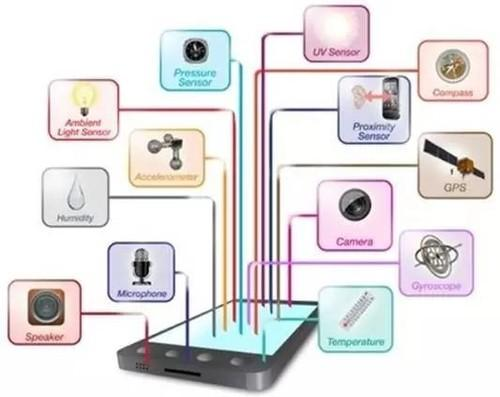
\includegraphics[width=0.6\textwidth]{image/1_3.jpeg}
    \caption{手机传感器类型}
\end{figure}

本文介绍了智能手机中常见的传感器类型，
包括运动传感器、环境传感器、生物识别传感器、成像与视觉传感器、接近和触控传感器，
以及声音与振动传感器。
每种传感器都在特定的应用场景中发挥了关键作用，
为用户带来了更流畅和高效的使用体验。同时，未来传感器的发展趋势如微型化、集成化、低功耗以及精度提升，将进一步推动手机功能的扩展，助力智能设备在物联网、健康监测等领域中的应用。

随着科技的不断进步，
智能手机中的传感器技术将更加智能化、个性化，为用户提供更加全面的服务。
这不仅会推动移动设备的持续创新，
还将使我们的日常生活更加便利和高效。
未来，传感器技术的发展潜力无穷，值得我们拭目以待。

\end{Answer}

\begin{question}{}{}
2、手机和外界互联的方法？
\end{question}
\begin{Answer}

\subsection*{引言}\noindent

在当今高度互联的社会中，
智能手机作为一种便捷的移动设备，
不仅用于通信，还通过多种方式与外界互联。
通过这些连接方式，手机能够访问互联网、传输数据、共享信息，并与其他设备或服务进行互动。
无论是通过蜂窝网络进行通话和数据传输，还是通过Wi-Fi、蓝牙等技术实现无线连接，
手机的互联功能已经渗透到我们生活的方方面面。

随着科技的快速发展，
智能手机与外界的连接方式也在不断丰富。
除了常见的无线和有线连接外，
云服务和卫星定位等技术也使手机可以随时随地获取数据，
提升了设备的功能性和便利性。
通过多样化的互联方式，手机成为了日常生活、工作、娱乐和社交中不可或缺的工具。

本文将详细介绍智能手机与外界互联的主要方式，
分析每种连接技术的应用场景及其未来发展趋势。

\subsection*{无线连接方式}\noindent

无线连接方式是智能手机与外界互联的主要方式之一，
提供了便捷的通信手段，
使用户能够在没有物理连接的情况下与互联网及其他设备进行数据传输。
主要的无线连接方式包括蜂窝网络、Wi-Fi、蓝牙和近场通信（NFC）。

\noindent\textbf{1. 蜂窝网络连接（3G/4G/5G）}\noindent

蜂窝网络是智能手机最常用的无线连接方式之一，
通过连接移动通信基站，手机可以进行语音通话、短信收发和数据传输。
随着移动通信技术的发展，蜂窝网络的速度和稳定性大幅提升，
特别是4G和5G网络的普及，带来了更快的下载速度、更低的延迟以及更广泛的覆盖。

\textbf{应用场景}：
\begin{itemize}
    \item \textit{语音通话和短信}：蜂窝网络是手机进行语音通话和短信发送的基础设施。
    \item \textit{移动数据服务}：3G、4G和5G网络支持高速的互联网连接，使用户能够随时随地进行网络浏览、流媒体播放和下载大文件。
    \item \textit{移动热点}：手机可以通过蜂窝网络共享其网络连接，作为移动热点为其他设备提供互联网接入。
\end{itemize}

\noindent\textbf{2. Wi-Fi}\noindent

Wi-Fi是一种基于无线局域网（WLAN）的通信技术，
允许智能手机通过无线方式连接至互联网。
Wi-Fi通常在家庭、公司、咖啡店等场所使用，
提供高速、低延迟的互联网连接。
相比蜂窝网络，Wi-Fi连接在本地网络中更加稳定且无额外数据流量费用。

\textbf{应用场景}：
\begin{itemize}
    \item \textit{家庭与公共网络接入}：用户可以通过Wi-Fi连接家中的路由器或公共Wi-Fi热点，享受高速的互联网服务。
    \item \textit{文件传输}：Wi-Fi支持高速文件传输，特别是在局域网内，手机与电脑或其他设备之间可以快速分享大文件。
    \item \textit{流媒体播放}：Wi-Fi提供的高带宽使得用户能够无缝播放高清视频和进行高质量的语音/视频通话。
\end{itemize}

\noindent\textbf{3. 蓝牙}\noindent

蓝牙是一种低功耗、短距离的无线通信技术，
主要用于设备之间的点对点连接。
蓝牙在音频设备、输入设备（如键盘、鼠标）和文件传输中被广泛应用。
现代智能手机支持多种蓝牙协议，允许连接无线耳机、蓝牙音箱、智能手表等设备。

\textbf{应用场景}：
\begin{itemize}
    \item \textit{无线音频传输}：蓝牙允许手机与无线耳机、音箱等设备连接，提供无缝的音频传输，尤其在音乐播放和语音通话中应用广泛。
    \item \textit{文件传输}：通过蓝牙，手机可以与其他设备（如电脑或手机）进行小文件的无线传输，适用于无网络环境下的近距离分享。
    \item \textit{外设连接}：蓝牙支持与智能手表、键盘、鼠标等外设连接，增强了手机的功能性。
\end{itemize}

\noindent\textbf{4. 近场通信（NFC）}\noindent

近场通信（NFC）是一种短距离的无线通信技术，通常在10厘米以内工作。
NFC的传输速度虽然不如Wi-Fi或蓝牙，
但其低功耗、快速配对和安全性使其广泛应用于移动支付、电子票务和设备快速配对等场景。

\textbf{应用场景}：
\begin{itemize}
    \item \textit{移动支付}：NFC技术支持快速、安全的移动支付，如Apple Pay、Google Pay等服务，使用户无需接触即可完成交易。
    \item \textit{快速设备配对}：通过NFC，用户可以快速将手机与蓝牙音箱、耳机等设备配对，无需复杂的手动操作。
    \item \textit{电子票务和门禁}：NFC可用于电子车票、门禁卡等应用，用户只需将手机靠近读卡器即可完成验证和支付。
\end{itemize}

\noindent\textbf{无线连接方式的优势}\noindent

无线连接方式大大提高了智能手机的便携性和使用灵活性。
通过无线技术，用户可以随时随地与互联网及其他设备连接，
享受高度的自由度和便捷性。
同时，随着5G和Wi-Fi 6等新一代技术的不断普及，
无线连接的速度和稳定性将进一步提升，
推动更多创新应用场景的出现。

\subsection*{有线连接方式}\noindent

虽然无线连接方式越来越普及，
但有线连接方式仍然是智能手机与外界互联的重要手段之一。
有线连接通常提供更高的数据传输速度、更稳定的连接以及充电功能。
常见的有线连接方式包括USB接口、OTG功能和HDMI/MHL连接。

\noindent\textbf{1. USB接口（USB-C/Lightning）}\noindent

USB接口是智能手机最常见的有线连接方式，
通常用于充电和数据传输。
现代手机大多采用USB-C接口，
而苹果设备则使用Lightning接口。
USB接口不仅支持与电脑等设备的高速数据传输，
还可以通过连接充电器进行快速充电。

\textbf{应用场景}：
\begin{itemize}
    \item \textit{数据传输}：通过USB接口，用户可以将手机与电脑连接，进行照片、视频、文件的高速传输。
    \item \textit{充电}：USB接口支持快速充电技术，用户可以通过连接适配器或移动电源为手机充电。
    \item \textit{外设连接}：通过USB接口，手机可以连接其他外设，如存储设备、相机等，实现数据同步或扩展功能。
\end{itemize}

\noindent\textbf{2. OTG（On-The-Go）}\noindent

OTG（On-The-Go）功能使智能手机可以直接连接并读取外部设备，
如U盘、键盘、鼠标等。通过OTG功能，
手机能够充当主机设备，
允许用户在没有电脑的情况下直接读取、传输文件，
甚至控制外部设备。

\textbf{应用场景}：
\begin{itemize}
    \item \textit{文件读取与传输}：通过OTG线缆，用户可以直接连接U盘或硬盘，访问、复制和传输文件，方便在无电脑时的存储操作。
    \item \textit{外设操作}：OTG支持连接外部键盘、鼠标，特别适用于需要更高效输入或控制的场景，如移动办公或游戏操作。
    \item \textit{摄影设备连接}：用户可以通过OTG将手机与相机连接，导出照片进行处理或分享，提升工作流程的便捷性。
\end{itemize}

\noindent\textbf{3. HDMI/MHL}\noindent

HDMI（High-Definition Multimedia Interface）和MHL（Mobile High-Definition Link）是手机与外部显示设备连接的有线方式。
通过这些接口，用户可以将手机屏幕镜像输出到电视、显示器等大屏设备上，
适用于播放视频、演示文稿或游戏投屏。

\textbf{应用场景}：
\begin{itemize}
    \item \textit{屏幕镜像}：通过HDMI或MHL连接，用户可以将手机屏幕投射到电视或投影仪上，用于观看视频、照片或进行演示。
    \item \textit{视频输出}：HDMI/MHL支持高清视频输出，适用于将手机作为媒体播放设备，直接连接到显示器或电视播放内容。
    \item \textit{游戏投屏}：游戏玩家可以通过这些接口将手机游戏投屏到大屏幕设备，提升游戏体验。
\end{itemize}

\noindent\textbf{有线连接方式的优势}\noindent

有线连接方式在数据传输速度和连接稳定性上具有明显优势。
与无线连接相比，
有线方式可以提供更高的带宽、更稳定的连接，
尤其在需要大容量数据传输或高清内容输出时表现出色。
此外，有线连接还可以兼顾充电功能，
确保设备在长时间使用中的续航能力。

随着技术的发展，
有线连接方式的速度和兼容性也在不断提升，
例如USB-C接口不仅支持更高的传输速率，
还具备了充电、数据传输与外设连接的多重功能。
虽然无线连接正在逐步取代部分有线功能，
但有线连接在某些高要求场景下仍不可替代。

\subsection*{云端服务互联}\noindent

随着云计算和云存储技术的快速发展，
智能手机通过云端服务实现了与外界的高效互联。
云端服务允许手机用户将数据存储在远程服务器上，
并通过互联网随时随地访问这些数据。
此外，云计算的强大处理能力也使得手机能够借助云端进行复杂的计算和处理任务。
主要的云端服务互联方式包括云存储和云计算。

\noindent\textbf{1. 云存储}\noindent

云存储（Cloud Storage）是将手机中的数据（如照片、视频、文档等）上传至云端服务器进行存储，
用户可以随时访问这些数据，而不必依赖本地存储空间。
这种方式不仅可以节省手机的存储空间，还提供了数据备份和跨设备同步功能，
方便用户在不同设备之间无缝使用同一份数据。

\textbf{应用场景}：
\begin{itemize}
    \item \textit{文件备份与恢复}：用户可以将重要文件（如照片、视频、联系人等）备份到云端，确保即使设备丢失或损坏，也能够随时恢复数据。
    \item \textit{跨设备同步}：通过云存储，用户可以在手机、平板、电脑等多个设备上同步文件，实现无缝的数据访问和管理。
    \item \textit{共享与协作}：云存储服务允许用户通过共享链接与他人分享文件，适合多人协作编辑文档、共享照片等场景。
\end{itemize}

\noindent\textbf{2. 云计算}\noindent

云计算（Cloud Computing）是通过互联网访问远程服务器的计算资源，
将复杂的计算任务转移至云端进行处理。
云计算为手机提供了强大的计算能力，
使其可以执行超出本地处理能力的任务，
如图像渲染、数据分析、视频编码等。
通过与云端的连接，手机用户可以享受云计算带来的高效性和低成本的计算资源。

\textbf{应用场景}：
\begin{itemize}
    \item \textit{云游戏}：云计算支持高要求的游戏场景，游戏的计算和渲染任务由云端服务器完成，用户只需通过手机进行操作和显示，减少了对本地硬件性能的依赖。
    \item \textit{云端渲染与编辑}：用户可以通过手机访问云端的图像或视频处理服务，将复杂的渲染或编辑任务转移至云端，尤其适合需要高性能计算的场景。
    \item \textit{远程办公与虚拟桌面}：云计算支持用户通过手机访问远程的虚拟桌面或办公环境，随时随地完成工作任务，特别适合移动办公场景。
\end{itemize}

\noindent\textbf{云端服务的优势}\noindent

云端服务互联为手机提供了强大的扩展能力，
不仅可以节省本地存储空间，
还可以借助云端的强大计算能力来完成复杂任务。
相比传统的本地存储和计算方式，
云端服务的优势在于灵活性、可扩展性和数据的跨设备访问。
通过云服务，用户无需担心存储空间不足或设备性能的限制，
能够随时享受高效、便捷的服务。

云端服务的普及改变了手机与外界互联的方式，
使其不仅仅是数据终端设备，
更是具备强大云端计算能力的智能终端。
未来，随着5G网络和边缘计算的发展，
云端服务的应用场景将进一步扩展，
带来更加高效的移动互联体验。

\subsection*{卫星定位与导航}\noindent

卫星定位与导航是智能手机与外界互联的一个关键功能，
广泛应用于地图导航、位置服务、运动追踪等场景。
通过连接全球导航卫星系统（GNSS），
智能手机能够实时获取其地理位置，
并为用户提供准确的定位信息。
常见的卫星定位系统包括GPS、北斗、GLONASS等。

\noindent\textbf{1. GPS（全球定位系统）}\noindent

GPS（Global Positioning System）是美国开发的全球卫星定位系统，
广泛应用于全球的定位和导航服务。智能手机通过接收GPS卫星发出的信号，
计算设备的具体位置。
GPS提供了高度精准的定位能力，
特别适合在开放环境下的户外活动，
如驾车导航、步行导航等。

\textbf{应用场景}：
\begin{itemize}
    \item \textit{地图与导航}：GPS被广泛应用于各种地图应用，如Google Maps、Apple Maps，为用户提供准确的实时位置和路线规划。
    \item \textit{运动追踪}：通过GPS，用户可以记录运动轨迹（如跑步、骑行），并分析速度、距离和路线。
    \item \textit{位置共享}：GPS定位功能支持用户在社交应用中与朋友或家人共享实时位置，方便聚会、行程安排等活动。
\end{itemize}

\noindent\textbf{2. 北斗卫星导航系统}\noindent

北斗卫星导航系统（BeiDou Navigation Satellite System，BDS）是中国开发的全球导航卫星系统，
作为GPS的补充和替代方案，
北斗在亚太地区尤其普及。
与GPS类似，北斗通过卫星信号为智能手机提供精准的定位服务，
提升了多区域的定位精度和覆盖范围。

\textbf{应用场景}：
\begin{itemize}
    \item \textit{全球导航}：北斗系统能够为全球用户提供精准的导航服务，特别是在中国及周边地区，北斗的定位精度更高。
    \item \textit{应急救援定位}：北斗系统的短报文通信功能允许用户在紧急情况下发送位置信息，适合偏远地区的应急救援。
    \item \textit{高精度位置服务}：北斗系统支持厘米级精度的定位，特别适合农业、工程测绘等需要高精度定位的领域。
\end{itemize}

\noindent\textbf{3. GLONASS}\noindent

GLONASS（Global Navigation Satellite System）是俄罗斯开发的全球卫星导航系统，
与GPS和北斗类似，GLONASS为智能手机提供全球定位服务。
GLONASS系统在极端条件下（如高纬度地区）的定位能力更强，
使其成为其他卫星系统的有力补充。

\textbf{应用场景}：
\begin{itemize}
    \item \textit{全球导航与定位}：GLONASS作为GPS的补充，提升了智能手机的全球定位精度，特别是在高纬度和极端环境下。
    \item \textit{增强的导航系统}：许多智能手机同时支持GPS、北斗和GLONASS多系统定位，通过组合多个系统信号，实现更高的定位精度和可靠性。
\end{itemize}

\noindent\textbf{4. 卫星定位与导航的协同工作}\noindent

现代智能手机通常支持多种卫星定位系统（如GPS、北斗、GLONASS等），
通过多重卫星信号的协同工作，
设备可以在不同环境中获得更高的定位精度和更广的覆盖范围。
特别是在城市环境或地理条件复杂的区域，
多系统协同定位能够有效减少误差，
提升导航的准确性和稳定性。

\textbf{优势}：
\begin{itemize}
    \item \textit{全球覆盖}：多种卫星系统的支持，确保了手机在全球范围内都能够获得可靠的定位服务。
    \item \textit{增强精度与稳定性}：通过结合不同卫星系统的信号，手机能够提供更精确的定位结果，特别是在高楼密集的城市或地理条件复杂的环境中。
\end{itemize}

\noindent\textbf{卫星定位与导航的未来发展}\noindent

随着技术的进步，卫星定位与导航的精度和速度将进一步提升。
新一代的卫星系统将能够提供更高的覆盖范围、更低的延迟和更高的定位精度，
特别是在5G和物联网的推动下，
卫星定位将在智能交通、无人驾驶、物流等领域发挥更加重要的作用。

\subsection*{未来发展趋势}\noindent

随着移动通信技术的不断进步，手机与外界互联的方式也在迅速演变。
未来的连接技术将更加注重速度、稳定性、安全性以及与新兴技术的深度融合。
以下是手机与外界互联的几大未来发展趋势。

\noindent\textbf{1. 5G网络与物联网（IoT）的融合}\noindent

5G网络的广泛部署正在改变手机与外界互联的模式。
5G不仅提供了超高速的互联网连接，
还具备低延迟和高设备密度支持的优势，使其成为物联网（IoT）发展的重要推动力。
手机将不再仅仅是一个通信工具，而是物联网生态中的核心节点，
能够与智能家居、智能交通、智能医疗等领域的数百亿设备实时互联。

\textbf{发展方向}：
\begin{itemize}
    \item \textit{超低延迟通信}：5G网络的低延迟特性将提升AR/VR体验、云游戏和无人驾驶等对实时性要求极高的应用场景。
    \item \textit{广泛的设备互联}：通过5G与物联网的结合，手机可以与多种智能设备实现无缝连接，助力智能家居、远程监控和智慧城市的建设。
\end{itemize}

\noindent\textbf{2. Wi-Fi 6和6E的普及}\noindent

随着Wi-Fi技术的迭代，Wi-Fi 6和即将普及的Wi-Fi 6E将成为未来手机无线连接的主流标准。
相比前几代Wi-Fi技术，Wi-Fi 6和6E不仅提供了更高的速度，
还在多设备连接和网络稳定性上表现更加出色，
特别是在拥挤的网络环境中能够提供更加稳定的性能。

\textbf{发展方向}：
\begin{itemize}
    \item \textit{更高带宽与稳定性}：Wi-Fi 6的高效数据处理能力，特别适用于多个设备同时连接的场景，增强了网络负载处理能力。
    \item \textit{6GHz频段的应用}：Wi-Fi 6E通过利用全新的6GHz频段，提供了更低的干扰和更高的数据传输速度，使其适用于未来的高带宽需求应用。
\end{itemize}

\noindent\textbf{3. 无线充电和反向充电的进步}\noindent
无线充电技术近年来取得了显著进步，
未来的手机将逐步摆脱有线充电的束缚，
依靠更高效、更快速的无线充电技术进行充电。
与此同时，反向充电技术的普及将使手机不仅能够为自身充电，
还可以为其他设备（如耳机、手表等）供电，提升了设备的互操作性。

\textbf{发展方向}：
\begin{itemize}
    \item \textit{更快的无线充电速度}：未来的无线充电技术将进一步提升功率，使其在充电速度上接近甚至超过有线充电。
    \item \textit{反向充电应用扩展}：反向充电不仅限于为小型设备充电，还可能扩展到更多设备，形成更加全面的能源共享生态。
\end{itemize}

\noindent\textbf{4. 多重生物识别技术的整合}\noindent

未来的手机将进一步整合多种生物识别技术，
如指纹识别、面部识别、虹膜识别、声纹识别等，
以提供更加安全、便捷的身份认证方式。
这些技术的融合不仅将增强设备的安全性，
还会为用户提供更好的体验，如更快的支付验证和设备解锁。

\textbf{发展方向}：
\begin{itemize}
    \item \textit{多模态生物识别}：通过将指纹、面部、虹膜等多种生物识别技术结合，提供更高的安全性和更少的误识别率。
    \item \textit{无缝身份验证}：未来生物识别技术将更加自然化、无感知，用户在操作手机时可以通过多个识别方式实现无缝的身份验证。
\end{itemize}

\noindent\textbf{5. 云计算和边缘计算的融合}\noindent

未来，手机不仅依赖于云端的计算能力，
还将借助边缘计算来提升数据处理的效率和速度。
边缘计算通过将计算资源分布在网络的边缘节点上，
减少了数据传输的延迟，使手机能够在复杂任务中快速响应。
这将特别适用于自动驾驶、智能医疗等需要高效实时计算的场景。

\textbf{发展方向}：
\begin{itemize}
    \item \textit{边缘计算的普及}：边缘计算将与云计算相结合，为手机提供更加智能的计算能力，特别是在对低延迟要求极高的应用场景中，如无人驾驶和智能城市。
    \item \textit{提升实时处理能力}：通过边缘计算，手机能够实时处理大量数据，减少对远程服务器的依赖，提升响应速度和效率。
\end{itemize}

\noindent\textbf{6. 安全与隐私保护技术的提升}\noindent

随着手机与外界的互联变得更加紧密，
安全和隐私保护成为未来发展的重要趋势。
手机将采用更为先进的加密技术、多重验证机制和隐私保护措施，
确保用户的数据在互联过程中免受攻击和泄露。
未来的隐私保护技术将涵盖从设备级别到应用层面的全面安全防护。

\textbf{发展方向}：
\begin{itemize}
    \item \textit{更强的数据加密}：未来手机将通过更高级别的加密技术（如量子加密）确保用户数据的安全传输和存储。
    \item \textit{分布式隐私保护}：在设备、应用和网络层面实现分布式的隐私保护，确保用户信息在不同场景下都能得到有效保护。
\end{itemize}

\noindent\textbf{总结}\noindent

未来手机与外界互联的技术将朝着更高速、更智能、更安全的方向发展。
5G网络、Wi-Fi 6、无线充电等技术将使手机的连接能力大幅提升；
而云计算、边缘计算与多重生物识别技术的融合将为用户带来更流畅的体验。
与此同时，随着隐私保护技术的不断进步，用户数据的安全性也将得到全面保障。
这些未来发展趋势将进一步推动智能手机的功能扩展与互联体验的提升。

\subsection*{结论}\noindent

智能手机作为现代生活中不可或缺的工具，
其与外界互联的方式极大地影响了用户的体验。
通过无线和有线连接，手机能够快速、便捷地与互联网、其他设备和云端服务进行交互；
通过卫星定位与导航，用户能够实时获取精准的地理位置；
而随着5G、物联网和云计算等技术的发展，
手机的互联方式将变得更加高效和多样化。

未来，随着5G网络的普及、Wi-Fi 6的应用以及物联网生态系统的逐步完善，
手机的互联功能将进一步扩展。
手机不仅可以作为用户的主要通信设备，
还将成为连接各种智能设备的核心枢纽，
推动智能家居、智慧城市和自动驾驶等新兴领域的发展。
同时，云端服务、边缘计算和多重生物识别技术的深度融合，
将带来更强大的计算能力和更安全的隐私保护。

总的来说，智能手机与外界的互联方式正在迅速演变，
未来的发展将为用户带来更加流畅、便捷和安全的使用体验。
随着技术的进步，手机将继续在生活、工作、娱乐等各个方面发挥更大的作用，
推动数字化社会的不断前进。

\end{Answer}

\begin{flushright}\begin{tabular}{rl}
  姓名: & 李俊洁\\
  班级: & 计算机2204 \\
  学号: & 20225443 \\
  课程: & 物联网导论 \\
  日期: & September 10, 2024 \\
  制作: & \LaTeX \\
  & 感谢您的批阅！
\end{tabular}\end{flushright}
\end{document}
